\begin{figure}[!t]
  \centering
  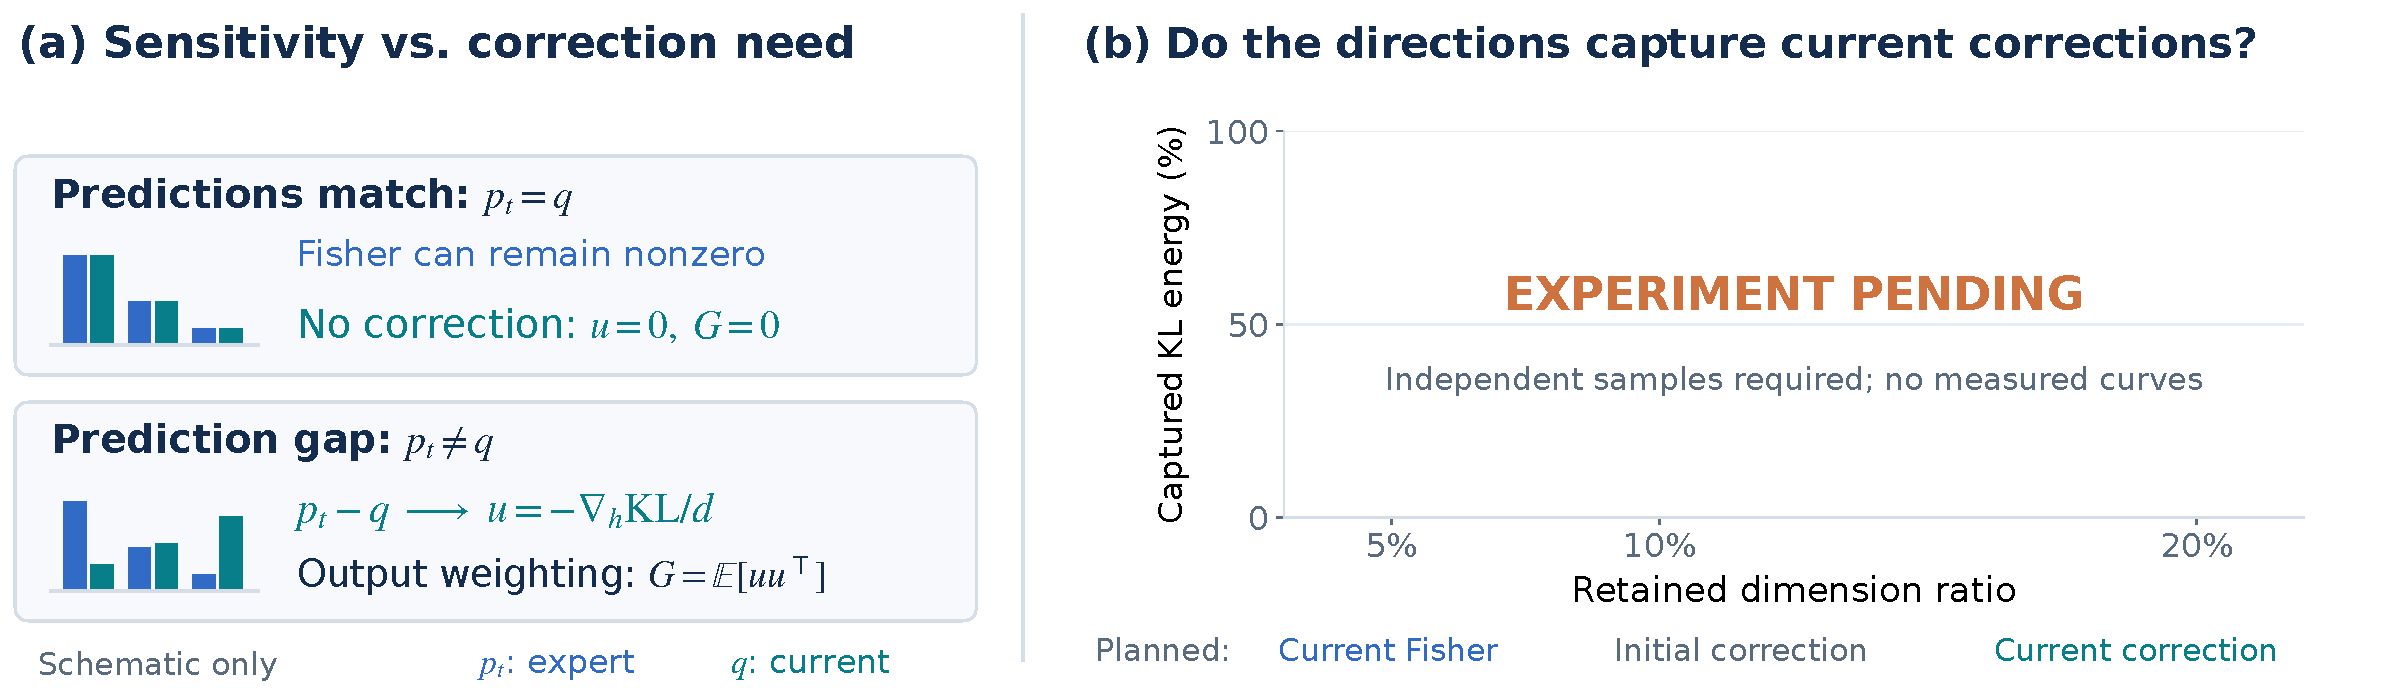
\includegraphics[width=\linewidth]{figures/ink_motivation.pdf}
  \caption{\textbf{局部敏感性不等于当前修正需求。}左：概念示意；当预测匹配时，Fisher 型几何仍可非零，而 KL 修正向量 $u$ 及其二阶矩 $G$ 为零；存在分歧时，残差经当前模型导数映射产生修正信号。右：独立样本修正能量捕获率的诊断版式，\textbf{实验待运行，无实测曲线}。此图不声称参数更新保证降低 KL。}
  \label{fig:ink-motivation}
\end{figure}
